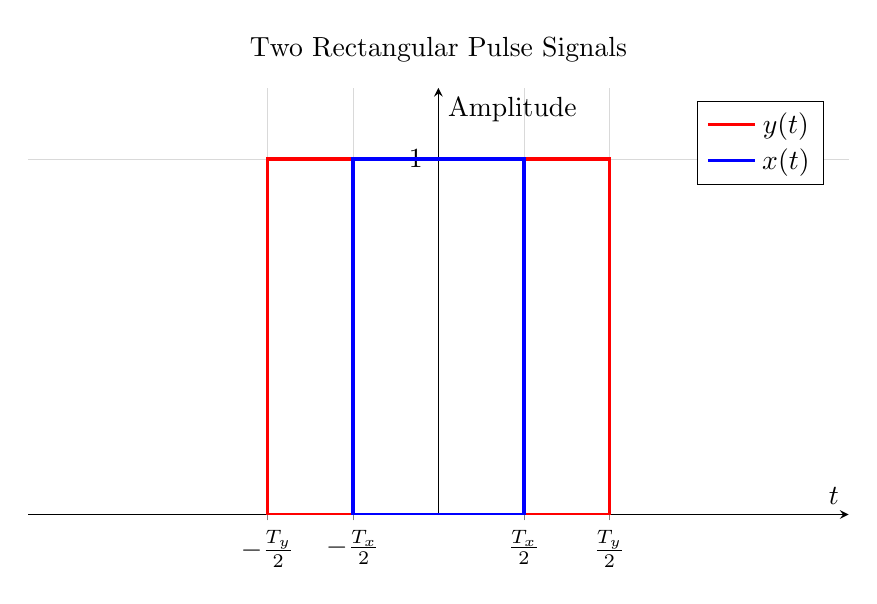
\begin{tikzpicture}
	\begin{axis}[
		% Set the overall style
		width=12cm,
		height=7cm,
		title={Two Rectangular Pulse Signals},
		xlabel={$t$},
		ylabel={Amplitude},
		% Position axes at the origin
		axis lines=middle,
		% Set axis limits to focus on the signals
		xmin=-0.6, xmax=0.6,
		ymin=0, ymax=1.2,
		% Set symbolic ticks for the pulse widths and amplitude
		xtick={-0.25, -0.125, 0.125, 0.25},
		xticklabels={$-\frac{T_y}{2}$, $-\frac{T_x}{2}$, $\frac{T_x}{2}$, $\frac{T_y}{2}$},
		ytick={1},
		yticklabels={$1$},
		% Add a grid
		grid=major,
		grid style={line width=.1pt, draw=gray!30},
		% Position the legend
		legend pos=north east,
		]
		
		% Use \addlegendimage to create legend entries for \draw commands
		\addlegendimage{red, very thick}
		\addlegendentry{$y(t)$}
		\addlegendimage{blue, very thick}
		\addlegendentry{$x(t)$}
		
		% Draw the wider pulse (y(t)) first so it's in the background
		\draw[red, very thick]
		(axis cs:-0.25, 0) -- (axis cs:-0.25, 1) -- (axis cs:0.25, 1)
		-- (axis cs:0.25, 0) -- cycle;
		
		% Draw the narrower pulse (x(t))
		\draw[blue, very thick]
		(axis cs:-0.125, 0) -- (axis cs:-0.125, 1) -- (axis cs:0.125, 1)
		-- (axis cs:0.125, 0) -- cycle;
		
	\end{axis}
\end{tikzpicture}